\begin{figure}[tbp]
\centering
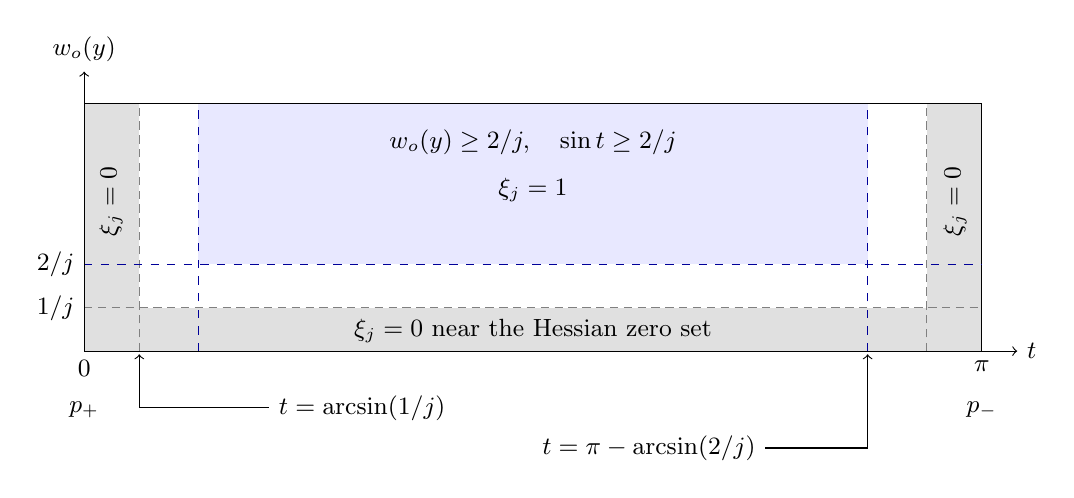
\begin{tikzpicture}[x=1cm,y=1cm,font=\small]
  \fill[gray!24] (0,0) rectangle (11.4,.55);
  \fill[gray!24] (0,.55) rectangle (.7,3.15);
  \fill[gray!24] (10.7,.55) rectangle (11.4,3.15);
  \fill[blue!9] (1.45,1.10) rectangle (9.95,3.15);
  \draw (0,0) rectangle (11.4,3.15);
  \draw[densely dashed,gray] (.7,0)--(.7,3.15);
  \draw[densely dashed,gray] (10.7,0)--(10.7,3.15);
  \draw[densely dashed,gray] (0,.55)--(11.4,.55);
  \draw[dashed,blue!60!black] (1.45,0)--(1.45,3.15);
  \draw[dashed,blue!60!black] (9.95,0)--(9.95,3.15);
  \draw[dashed,blue!60!black] (0,1.10)--(11.4,1.10);
  \node at (5.7,2.05) {$\xi_j=1$};
  \node[align=center] at (5.7,2.65)
    {$w_o(y)\ge 2/j,\quad \sin t\ge 2/j$};
  \node at (5.7,.26) {$\xi_j=0$ near the Hessian zero set};
  \node[rotate=90] at (.34,1.9) {$\xi_j=0$};
  \node[rotate=90] at (11.06,1.9) {$\xi_j=0$};
  \draw[->] (0,0)--(11.85,0) node[right] {$t$};
  \draw[->] (0,0)--(0,3.55) node[above] {$w_o(y)$};
  \node[below] at (0,0) {$0$};
  \node[below] at (11.4,0) {$\pi$};
  \node[left] at (0,.55) {$1/j$};
  \node[left] at (0,1.10) {$2/j$};
  \node[below,align=center] at (0,-.52) {$p_+$};
  \node[below,align=center] at (11.4,-.52) {$p_-$};
  \draw[<-] (.7,-.04)--(.7,-.72)--(2.35,-.72)
    node[right] {$t=\arcsin(1/j)$};
  \draw[<-] (9.95,-.04)--(9.95,-1.23)--(8.65,-1.23)
    node[left] {$t=\pi-\arcsin(2/j)$};
\end{tikzpicture}
\caption{The product cutoff on a suspended component.  The horizontal
variable is the suspension angle in
$\Phi(t,y)=(\sin t\,y,\cos t)$; the two end slices collapse to the
tips $p_+$ and $p_-$.  The vertical variable records the value of
$w_o(y)$, not a coordinate on $\Omega_o$.  Gray regions have
$\xi_j=0$, and the blue region has $\xi_j=1$; the intervening bands
contain the smooth transitions.  The scales are schematic, and no
shape or regularity of the Hessian zero set is represented.}
\label{fig:suspension-cutoff}
\end{figure}
